\chapter{Introduction}
In this course we will be concerned with ordinary differential equations, ODEs.

\begin{defin}
An ordinary differential equation (ODE) is a differential equation containing one or more functions of \underline{\textbf{exactly one}} independent variable and its derivatives.
\end{defin}

ODEs relate the change of one variable to changes in another variable and can be used to model and understand a wide variety of phenomena, such as projectile motion, animal population interactions and the progression of chemical reactions.

In these notes we consider two important aspects in the theory of ordinary differential equations. Specifically, we seek to
\begin{enumerate}
\item develop methods of modelling physical phenomena;
\item understand the properties of the equations without explicitly solving them.
\end{enumerate}

Point 2 may seem counter-intuitive as we have a variety of techniques that enable us to solve ODEs in closed form. Further, even if an explicit solution is not available, we can use numerical simulations to illustrate the dynamics of the ODEs. However, direct solutions are not always possible and, even when they are, they may not always enable clear interpretations and understanding of the underlying system. Equally, our analytical techniques will give us confidence in the solutions produced by numerical software.

Critically, what we gain in analytical specificity, we lose in global accuracy. Namely, we are going to learn techniques that will allow us to rigorously examine small regions of the ODE space at the expense of losing knowledge of the global dynamics. However, by the end of the course we will be able to patch together multiple parts of the local analysis in order to give us an approximate understanding of the entire dynamical system.

\section{Preliminary definitions}
We will be considering the rate of change of a variable, $u$, with respect to another variable, $t$. This dependence will be denoted
\bb
u(t).
\ee
Here, $u$ is a scalar function (\ie one-dimensional), but more generally, we will be considering systems of variables
\bb
\bm{u}(t)=\l u_1(t),u_2(t),\dots,u_k(t)\r.
\ee
On the board we will usually write bold symbols with an underline\footnote{I was once told that we use underlines to illustrate bold variables because when typesetting a document an underline would tell the printer that that symbol needed to be bold. However, if this is true, how did the writer indicate that they wanted a symbol underlined?} as it is easier to see, thus, $\bm{u}=\underline{u}$.

The values of $u$ or $\bm{u}$ define quantities of interest. For example they could be an animal population density, a distance or a speed. Further, $t$ can be any variable which these quantities are dependent on. Generally, however, we will take $t$ to be time and we will be considering how these values temporally evolve.

In order to link the changes in these quantities we define a system of ODEs in the most general way possible,
\bb
\bm{F}\l t,\bm{u},\frac{\rd \bm{u}}{\rd t},\frac{\rd^2 \bm{u}}{\rd t^2},\dots,\frac{\rd^n \bm{u}}{\rd t^n}\r=0,
\ee
with initial condition given by
\bb
\bm{u}(0)=\bm{u}_0.
\ee
Note that the initial condition is kept general as we will usually be interested in how the dynamics of the system change for different starting points.

\begin{example}[frametitle=Bacteria population growth]
\label{Expo_growth}
\COL{In this case we are only considering one population, thus, $\bm{u}=u$ and we specify $u(t)$ to be the population of E.Coli at time $t$. Initially, the population is $u_0$ and resources are abundant, thus, each E.Coli is able to double itself at a rate $r$/s. Explicitly, the population grows at a rate proportional to the population already present, \ie
\bb
\frac{\rd u}{\rd t}=ru.
\ee
This equation can be trivially solved to give
\bb
u(t)=u_0\exp(rt),\label{Intro_exp}
\ee
see \fig{Exponential}.

Note instead of specifying the time at which a population takes an arbitrary value, we can consider the more general time scale of how long does it take the population to double? Namely, at what point, $t_2$, is $u(t_2)=2u_0$. Rearranging \eqn{Intro_exp} we derive that
\bb
t_2=\frac{1}{r}\log\l 2\r.
\ee

Critically, once a model is constructed and an answer is found, we must consider whether if it is a good model or not. Clearly this model has problems because it predicts the population will grow exponentially quickly, without bound. The key problematic assumption that we have made is that the resources (\eg space, nutrients, etc.) do not run out. Although this may be a fine assumption to begin with, eventually the bacteria will be limited by competition.}
%\begin{figure}[!!!h!!!tb]
{\centering
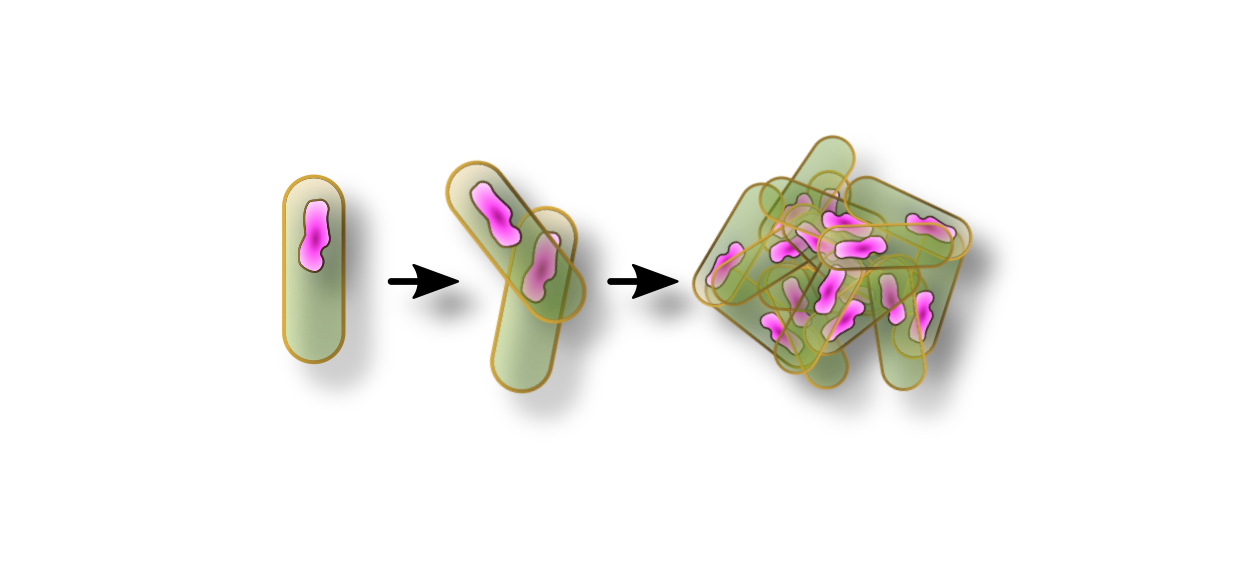
\includegraphics[width=\textwidth]{../Pictures/Bacteria.png}}
%\end{figure}
\end{example}


\begin{example}[frametitle=Bacteria and nutrient populations.]\label{Logi_growth}
\COL{Imagine a case similar to the one above, but we introduce a nutrient population, $v$. We assume that a bacterium can divide at a rate $r$ if and only if it can interact with enough nutrient. However, the nutrient is depleted at a rate $r$ as the bacteria interacts with it.

Here, the equation governing this system is going to be provided. However, later on we will learn how to write down and interpret interaction equations of the form
\bb
u+v \stackrel{r}{\longrightarrow} 2u.
\ee

The governing equations are
\begin{align}
\frac{\rd u}{\rd t}&=ruv,\quad u(0)=u_0,\label{Pop_u}\\
\frac{\rd v}{\rd t}&=-ruv,\quad v(0)=v_0.
\end{align}}
\COL{We notice that we can add the two equations and integrate to provide a conserved quantity,
\bb
u+v=c.\label{Conserved_c}
\ee
We can substitute \eqn{Conserved_c} into \eqn{Pop_u} to get
\bb
\frac{\rd u}{\rd t}=ru(c-u).\label{Log_1}
\ee
This is known as the logistic equation and we will see it many times throughout these notes, it is a simple example of competition between species for resources.}

\COL{Using partial fractions, we can directly solve \eqn{Log_1}. Specifically,
\begin{align}
\frac{\rd u}{\rd t}&=rcu\l 1-\frac{u}{c}\r,\nonumber\\
\Rightarrow\int_0^T\frac{\rd u}{u(1-u/c)}&=\int_0^Trc \rd t,\nonumber\\
\Rightarrow\int_0^T \frac{1}{u}+\frac{1/c}{1-u/c}  \rd u&=rcT,\nonumber\\
\Rightarrow\left[\ln(u)-\ln\l 1- \frac{u}{c} \r \right]^T_0&=rcT,\nonumber\\
\Rightarrow\ln\l\frac{u}{1- \frac{u}{c}} \r-\ln\l\frac{u_0}{1- \frac{u_0}{c}} \r&=rcT,\nonumber\\
\Rightarrow u(T)=\frac{c}{1+\frac{c-u_0}{u_0}\exp\l{-rcT}\r},
\end{align}
see \fig{Logistic}.

Comparing the models of bacteria growth, illustrated in \fig{Growth_examples}, we see that \eqn{Log_1} is a more realistic model for growth because there is a maximum population value which can be supported by the experiment. This maximum value is given by $c$ and is known as the carrying capacity. The parameter grouping $rc$ is also important as this control the time scale over which this maximum is obtained.}
\end{example}
\begin{figure}[!!!h!!!tb]
{\centering
\subfigure[\label{Exponential}]{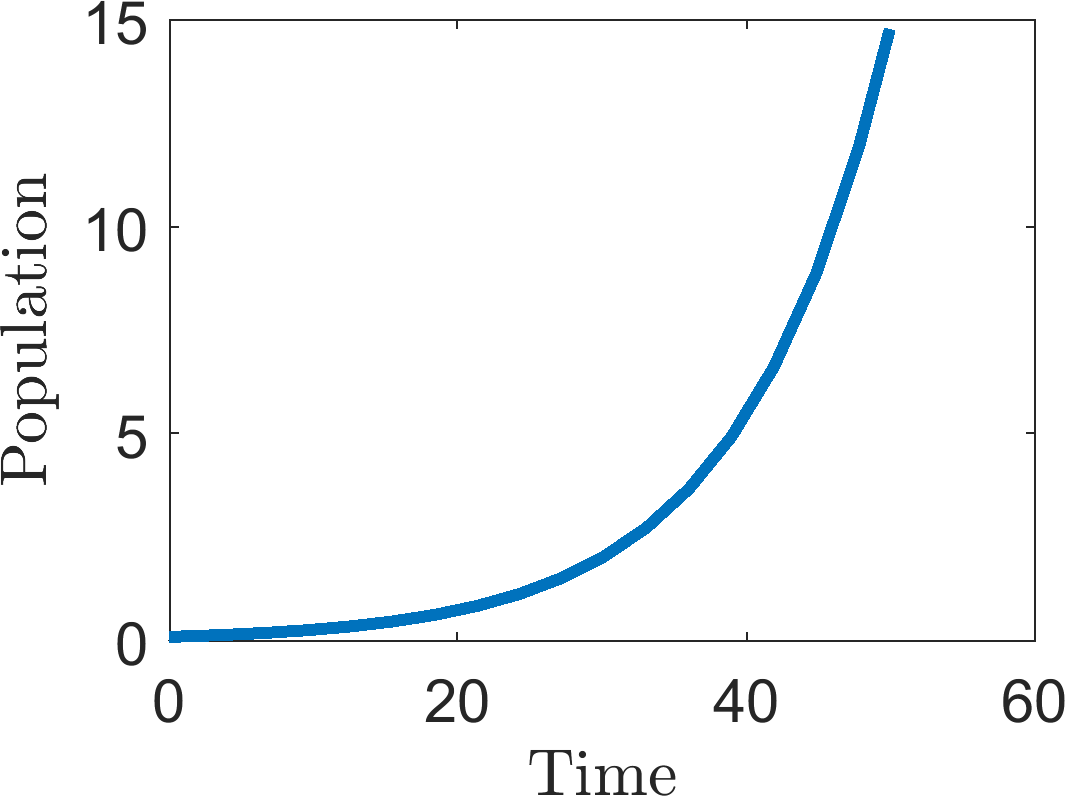
\includegraphics[width=\ttp]{../Pictures/Exponential.png}}
\subfigure[\label{Logistic}]{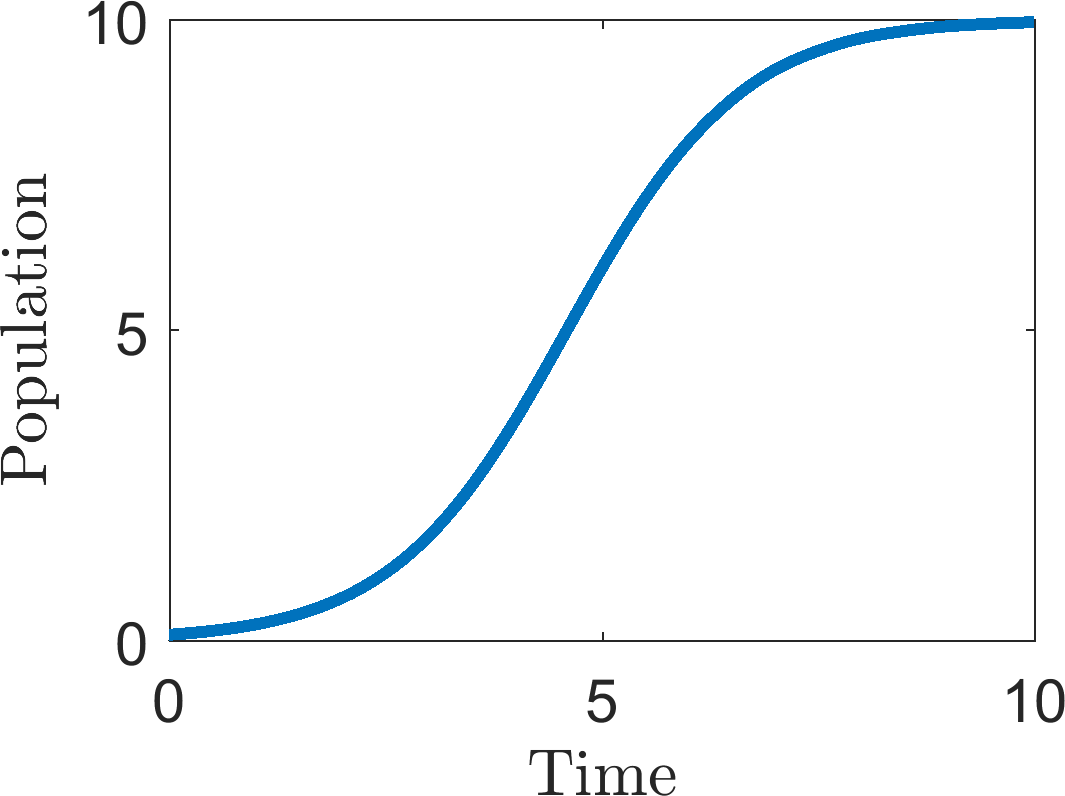
\includegraphics[width=\ttp]{../Pictures/Logistic.png}}
\caption{(a) Exponential growth. Parameters are $r=u_0=0.1$. See example \ref{Expo_growth}. (b) Logistic growth. Parameters are $c=10$, $r=u_0=0.1$. See example \ref{Logi_growth}.}\label{Growth_examples}}
\end{figure}


\begin{example}[frametitle=Duffing's equations.]\label{Duffing_example}
For our last example, consider the Duffing oscillator. The equation is simply a toy example that can be used to examine complex phenomena in a simple equation. In terms of interpretation, you can think of the equation as modelling the displacement of a beam near two magnetics. Critically, the beam and magnets are being forced to oscillate with amplitude $\gamma$ and frequency $\omega$ \see{Duffing_beam}.
\bb
\underbrace{\frac{\rd^2 x}{\rd t^2}}_{\textrm{Acceleration}}+\underbrace{2\delta\frac{\rd x}{\rd t}}_{\textrm{Air resistance}}+\underbrace{\beta x+\alpha x^3}_{\textrm{Beam's restorative force}}=\underbrace{\gamma\cos(\omega t)}_{\textrm{Forcing term}}.\label{Duffing_eqn}
\ee

We are not going to try and analytically solve or analyse Duffing's equation. Instead, we illustrate the dynamics that the equation produces as the amplitude of oscillation, $\gamma$, increases. Specifically, as $\gamma$ is increased the system becomes chaotic \see{Duffing_equation}.
\end{example}
\begin{figure}[!!!h!!!tbp]
\centering
\subfigure[\label{Duffing_beam}]{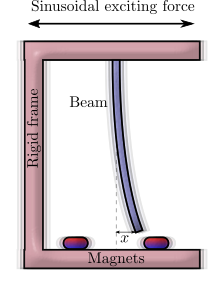
\includegraphics[width=.3\textwidth]{../Pictures/Duffing_beam.png}}
\subfigure[\label{Duffing_equation}]{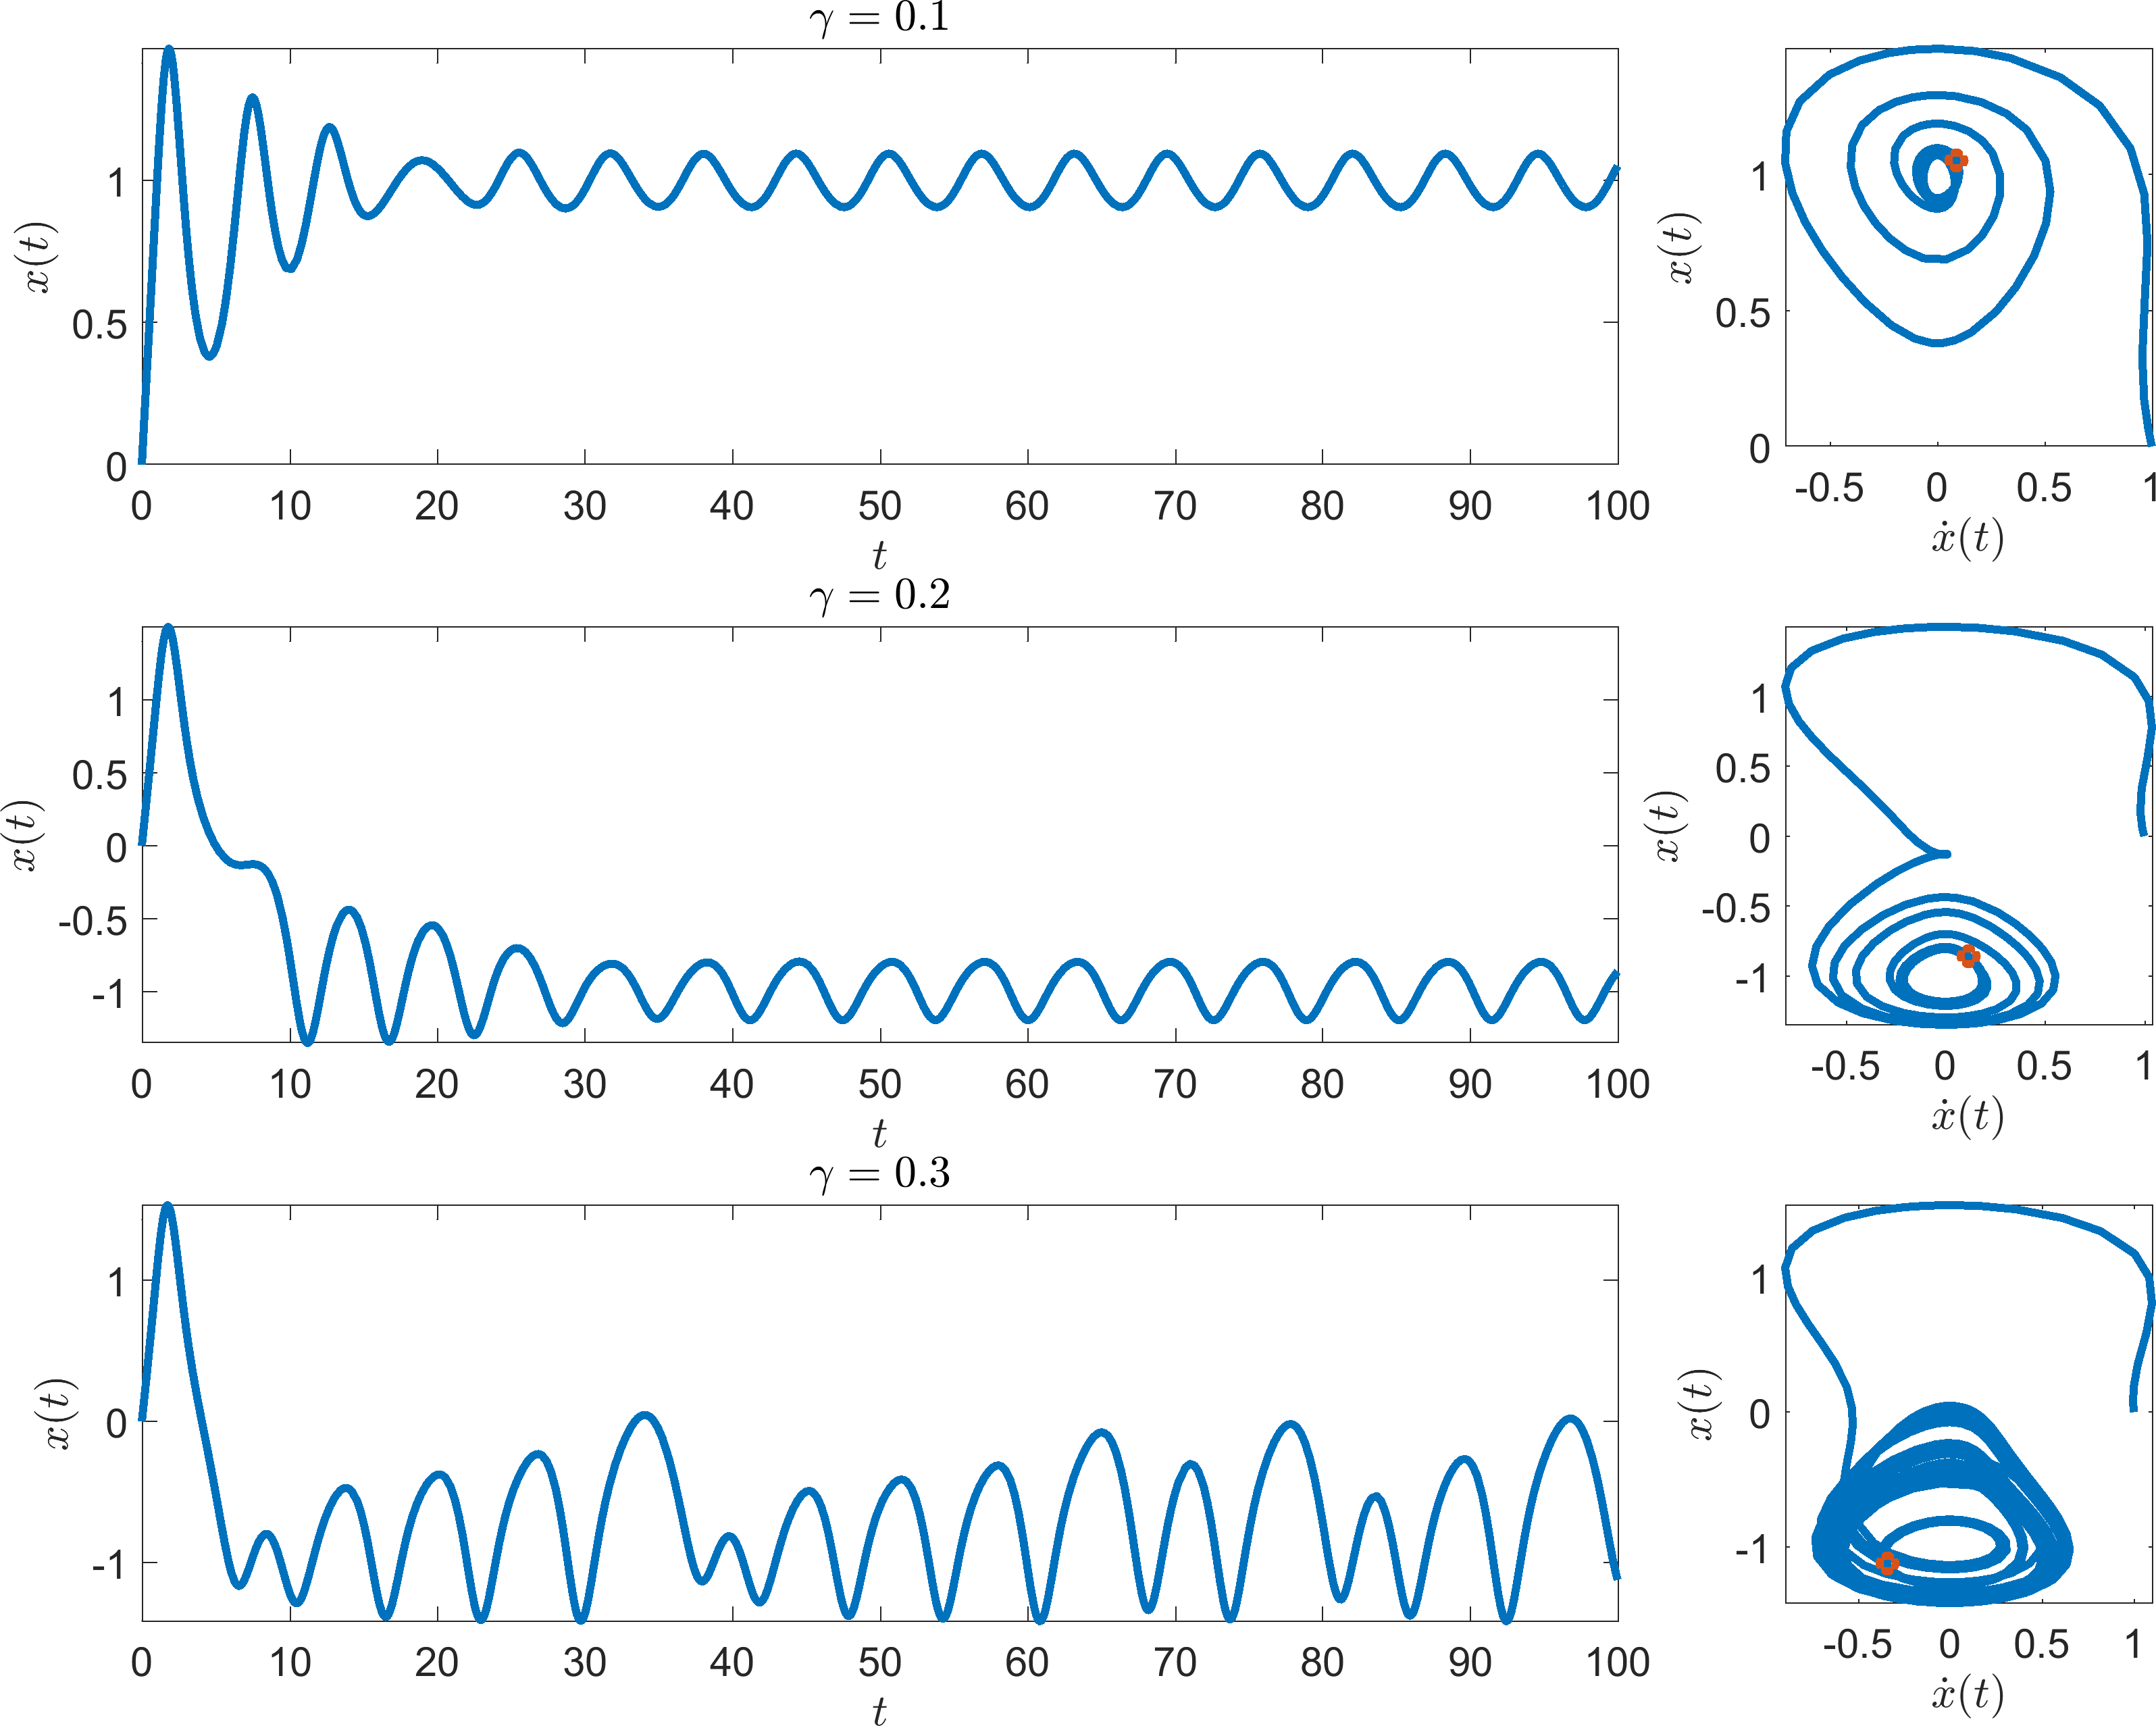
\includegraphics[width=\textwidth]{../Pictures/Duffing.png}}
\caption{\label{Duffing}(a) Schematic diagram of the system underlying Duffing's equation. (b) Three simulations of \eqn{Duffing_eqn} with increasing values of $\gamma$.}
\end{figure}

\begin{defin}
The \textbf{order} of a differential equation is the value of the highest derivative in the equation.
\end{defin}
Examples \ref{Logi_growth} and \ref{Expo_growth} are both first order equations, whilst example \ref{Duffing_example} is a second order equation. Generally (like polynomial equations of order) a differential equation of order $n$ will have $n$ linearly independent solutions.

\begin{defin}
A system of differential equations is \textbf{autonomous} if the system does not explicitly depend on the independent variable.
\end{defin}
When the variable is time, they are also called time-invariant systems, this simply means that we are assuming that the defined underlying laws of the system are identical to those for any point in the past, or future.

\begin{defin}
To save time we use a dot or prime mark to denote a derivative with respect to the argument, thus,
\bb
\dot{\bm{u}}(t)=\bm{u}'(t)=\frac{\rd \bm{u}}{\rd t}.
\ee
\end{defin}
Traditionally, dots are primarily used when the variable is time and primes are used otherwise. Note that higher orders derivatives are signified by the appropriate number of dots or primes. Namely, a second derivative would be denoted by two dots or primes, etc.

\begin{defin}
A \textbf{trajectory} is a solution, $u(t)$.
\end{defin}
The graphs in \figs{Growth_examples}{Duffing} illustrate single trajectories of their respective systems.



In this course we are going to occupy ourselves with systems of autonomous first order equations, of the form
\bb
\frac{\rd \bm{u}}{\rd t}=\dot{\bm{u}}=\bm{F}(\bm{u}).\label{ODE}
\ee
This may seem highly restrictive. However, systems of first order equations can have extremely complicated properties, such as oscillations and chaos, which we will try to understand.

\COL{Critically, equations of higher order can be written as a system of first order equations. For example, if
\bb
\bm{G}\l \bm{u},\frac{\rd \bm{u}}{\rd t},\frac{\rd^2 \bm{u}}{\rd t^2},\dots,\frac{\rd^n \bm{u}}{\rd t^n}\r=0
\ee
then we can define $n-1$ new equations of the form $\bm{v}_1=\rd \bm{u}/\rd t$ and $\bm{v}_i=\rd \bm{v}_{i-1}/\rd t=\rd^{i} \bm{u}/\rd t^{i}$ for $2\leq i \leq n-1$ to produce the first order system
\begin{align}
&\bm{G}\l \bm{u},\bm{v}_1,\dots,\bm{v}_{n-1},\frac{\rd \bm{v}_{n-1}}{\rd t}\r=0,\\
&\frac{\rd \bm{u}}{\rd t}=\bm{v}_1,\\
&\vdots\nonumber\\
&\frac{\rd \bm{v}_{n-2}}{\rd t}=\bm{v}_{n-1}.
\end{align}}
\begin{example}[frametitle=Duffing's equations without forcing.]\label{Duffing_example2}
\COL{Setting $\gamma=0$ in Duffing's equation and letting
\bb
v=\frac{\rd x}{\rd t}
\ee
then we are able to convert the single second order equation seen in \eqn{Duffing_equation} to two first}\COL{ order ODEs,
\begin{align}
\frac{\rd v}{\rd t}&=-2\delta v-(\beta x+\alpha x^3)\\
\frac{\rd x}{\rd t}&=v.
\end{align}
Note that $v$ is an apt variable name for the variable, because, as discussed in example \ref{Duffing_example}, $x$ can be thought of as position, making $v$ a velocity.}
\end{example}
\begin{thm}
A solution trajectory, $\bm{u}(t)$, of \eqn{ODE} cannot self-intersect \see{Trisectrix}.
\end{thm}
\begin{proof}
\COL{Suppose there is an intersection. Hence, there exist two points, $t_1$ and $t_2$, such that $\bm{u}(t_1)=\bm{u}(t_2)$ then we will also have that $\bm{F}(\bm{u}(t_1))=\bm{F}(\bm{u}(t_2))$. However, the curves intersect, thus, the curves must be travelling in different directions at $t_1$ and $t_2$ \see{Intersect}, meaning that the derivatives are different there, \ie $\dot{\bm{u}}(t_1)\neq\dot{\bm{u}}(t_2)$. But
\bb
\dot{\bm{u}}(t_1)=\bm{F}(\bm{u}(t_1))=\bm{F}(\bm{u}(t_2))=\dot{\bm{u}}(t_2),
\ee
which produces a contradiction. Hence the curves cannot intersect.}
\end{proof}
\begin{figure}[!!!h!!!tb]
\centering
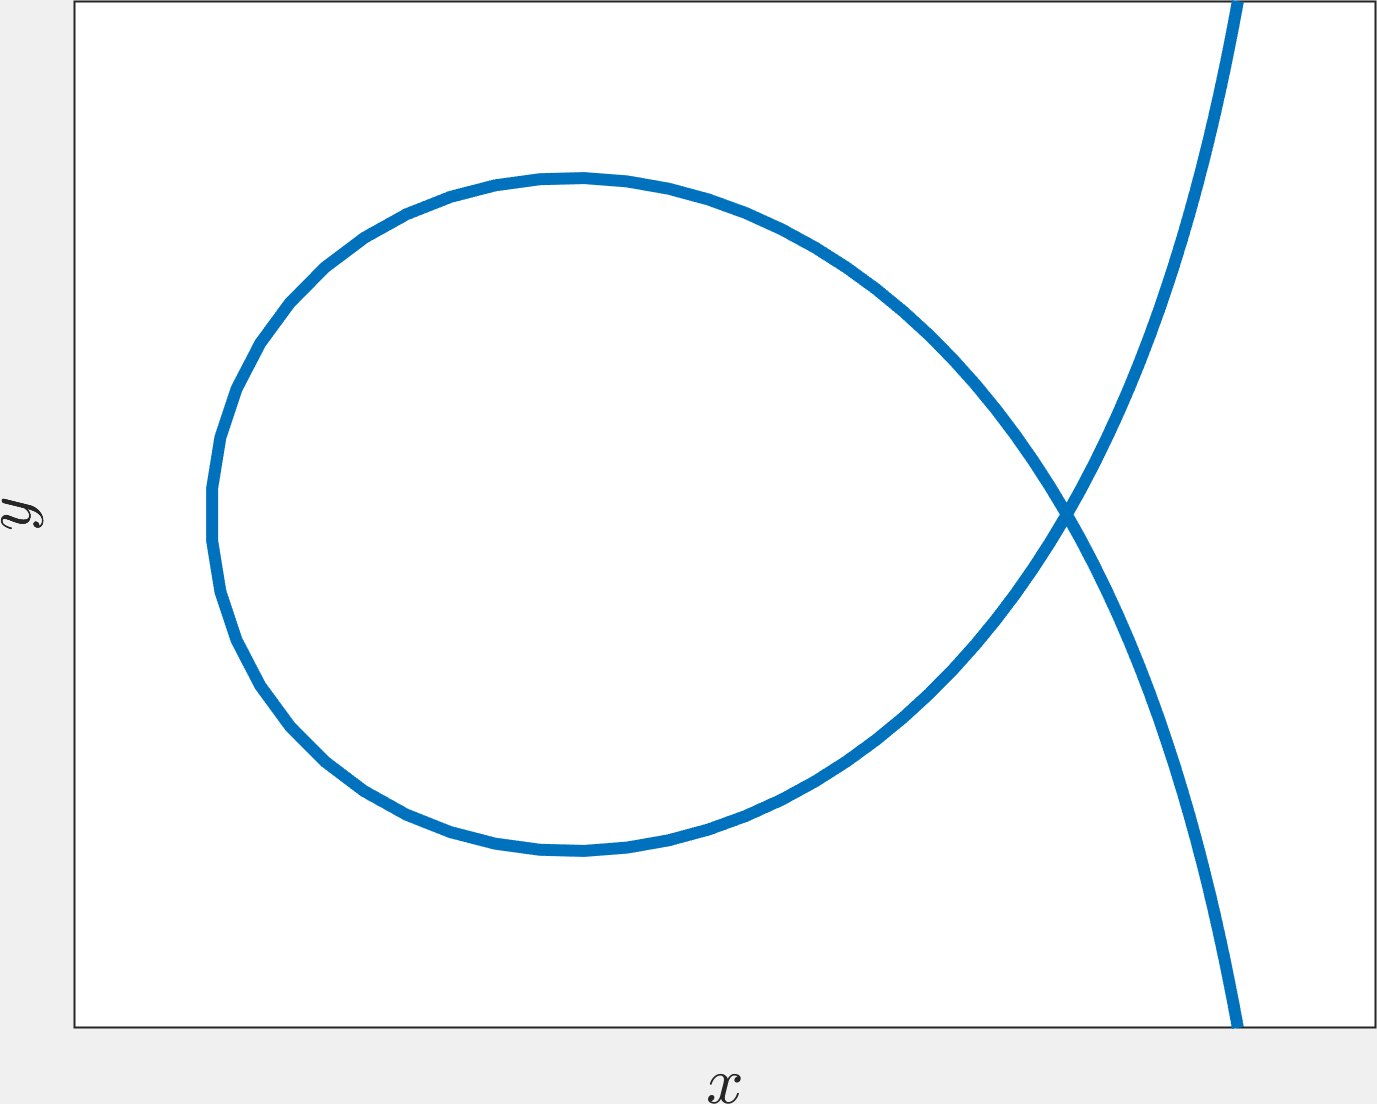
\includegraphics[width=\ttp]{../Pictures/Trisectrix.png}
\caption{\label{Trisectrix} A solution of \eqn{ODE} cannot look like this.}
\end{figure}


\subsection{Existence and uniqueness}
With this being an applied mathematics course we are often very `fast and loose' with our rigour. However, it is good to know that theorems have been proven regarding the existence and unique of solution to \eqn{ODE}. Here we will quote the theorem in one dimension, but the theorem can be expanded to any number of variables.
\begin{thm}Existence-Uniqueness theorem.

Suppose the function $F(u)$ is differentiable and the derivative, $F'(u)$, is continuous for all values of $u$ then there will exist some constant $c>0$ such that
\bb
\dot{u}=F(u),\quad u(t_0)=u_0,
\ee
has a solution and it is guaranteed to exist and be unique in some finite time interval $|t-t_0|<c$.\label{Existence_Uniqueness}
\end{thm}
Note that:\COL{
\begin{itemize}
\item we will not consider the proof here. For those who are interested look up ``Picard's theorem''. Picard's theorem is actually weaker than the one specified above, but theorem \ref{Existence_Uniqueness} expresses the statement in the most useful form for us.
\item in many cases solutions will exist and be unique for all time, but, the theorem hardly ever provides an optimal value for $c$. However, the theorem is general enough to include cases where `blow up' occurs. Namely, blow up occurs when a solution tends to infinity in finite time.
\item without loss of generality we can always take $t_0=0$ (why?). \textbf{This is only true in autonomous systems}.
\item solution curves cannot intersect, otherwise there would be two different solutions going through the same point and there would not be uniqueness around the intersection \see{Intersect}.
\item the case for higher dimensional systems is effectively the same except we need the function
\bb
\bm{F}(\bm{u})=\left(
\begin{array}{c}
{F_1}(u_1,u_2,u_3,\dots,u_n)\\
{F_2}(u_1,u_2,u_3,\dots,u_n)\\
\vdots\\
{F_n}(u_1,u_2,u_3,\dots,u_n)
\end{array}
\right)
\ee to be continuous in all of its derivatives.
\end{itemize}}
\begin{figure}[!!!h!!!tb]
\centering
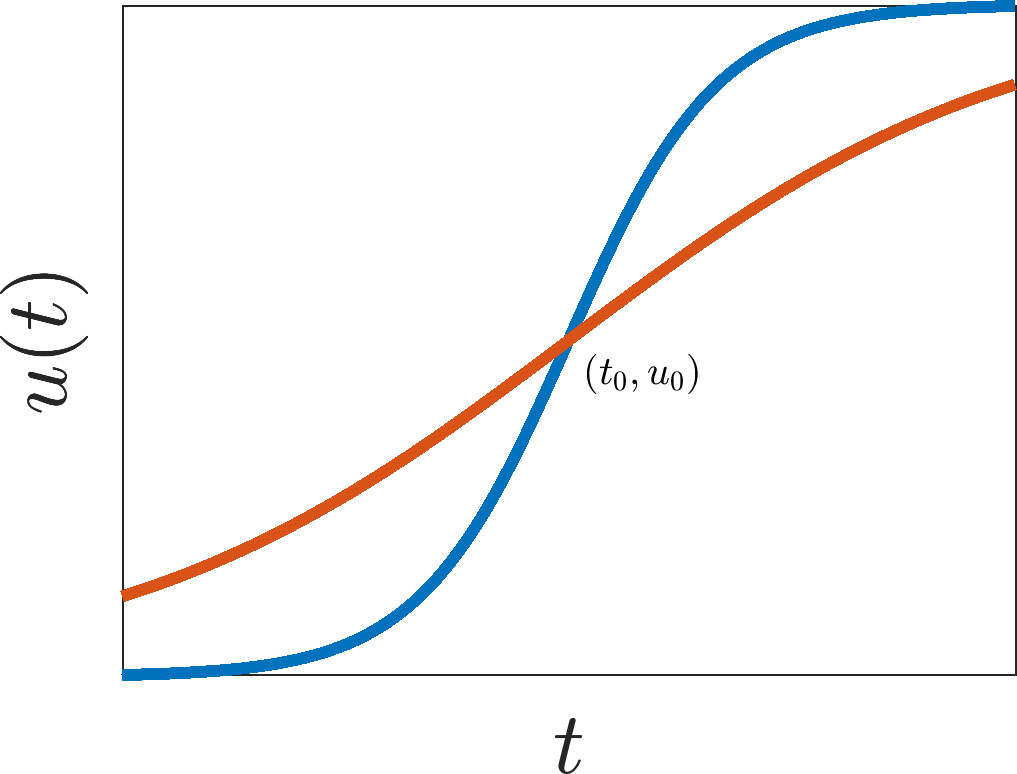
\includegraphics[width=\ttp]{../Pictures/Intersection.png}
\caption{\label{Intersect}Two different solution curves of a one-dimensional ODE cannot intersect.}
\end{figure}

\begin{defin}\label{Monotonic_def}
A differentiable function is \textbf{monotonic} if its derivative never changes sign. Moreover, the function is monotonically increasing (decreasing) if the derivative is positive (negative).
\end{defin}
\begin{defin}\label{Strict_monotonic_def}
A differentiable function is \textbf{strictly monotonic} if its derivative never changes sign and is never zero.
\end{defin}
See \fig{Monotonics} for examples of definitions \ref{Monotonic_def} and \ref{Strict_monotonic_def}.
\begin{figure}[!!!h!!!tb]
\centering
\subfigure[\label{Non_monotonic}]{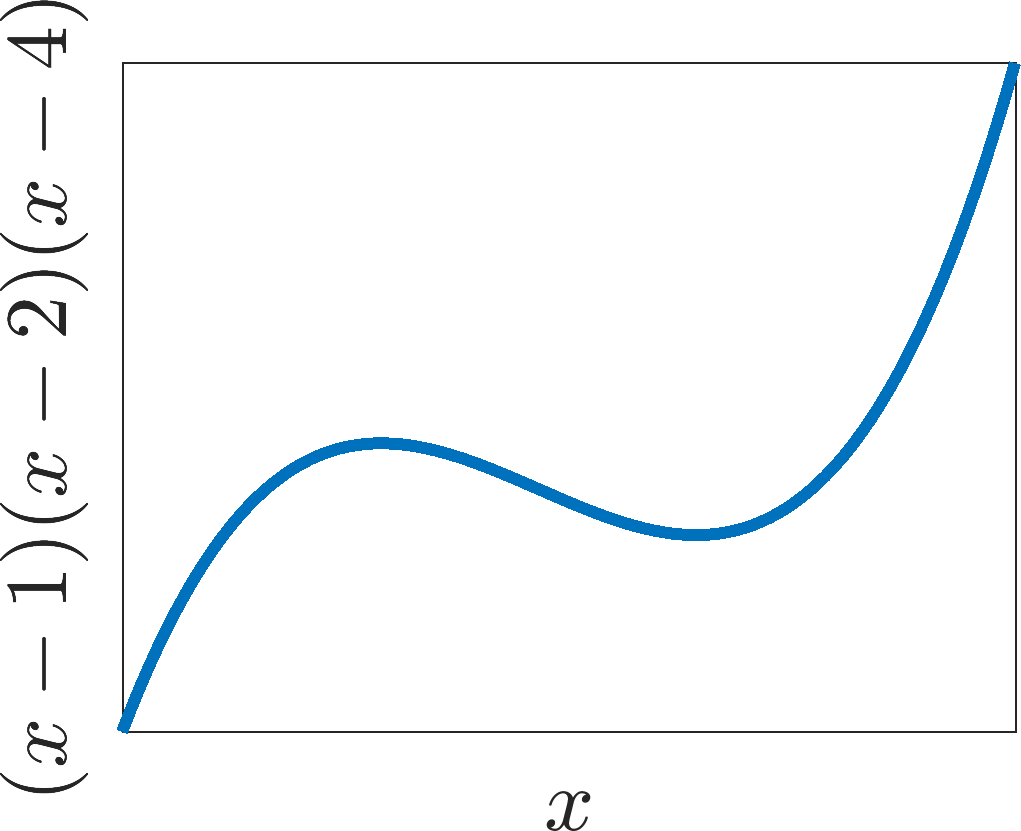
\includegraphics[width=\tttp]{../Pictures/Non_monotonic.png}}
\subfigure[\label{Monotonic}]{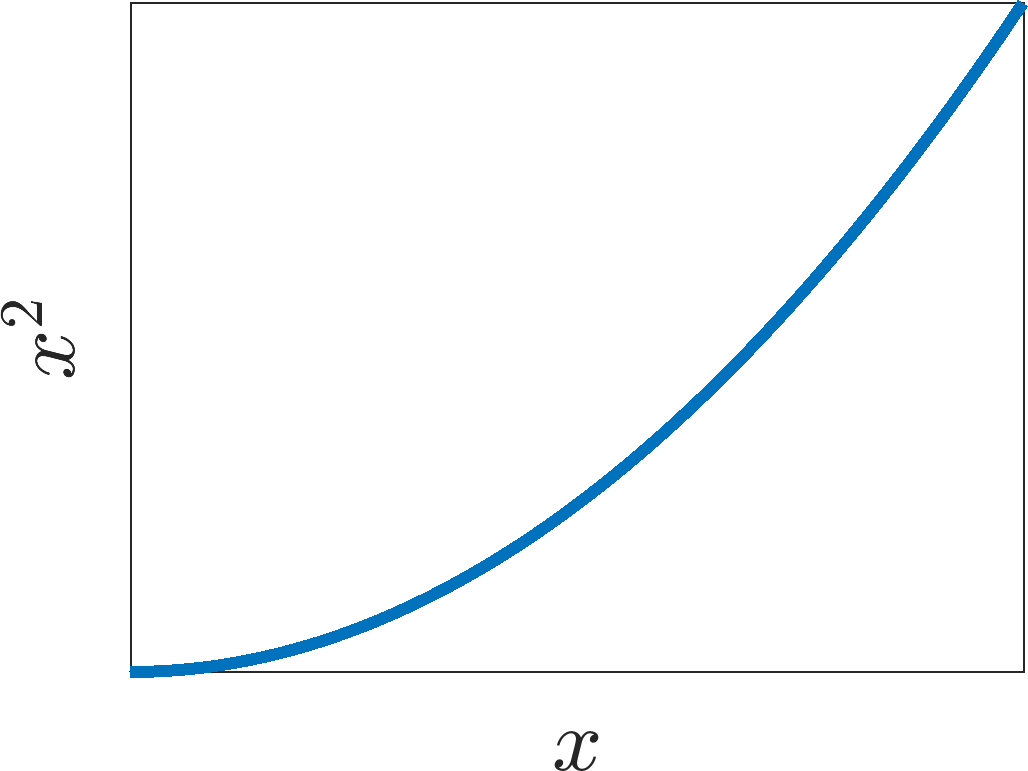
\includegraphics[width=\tttp]{../Pictures/Monotonic.png}}
\subfigure[\label{Strictly_monotonic}]{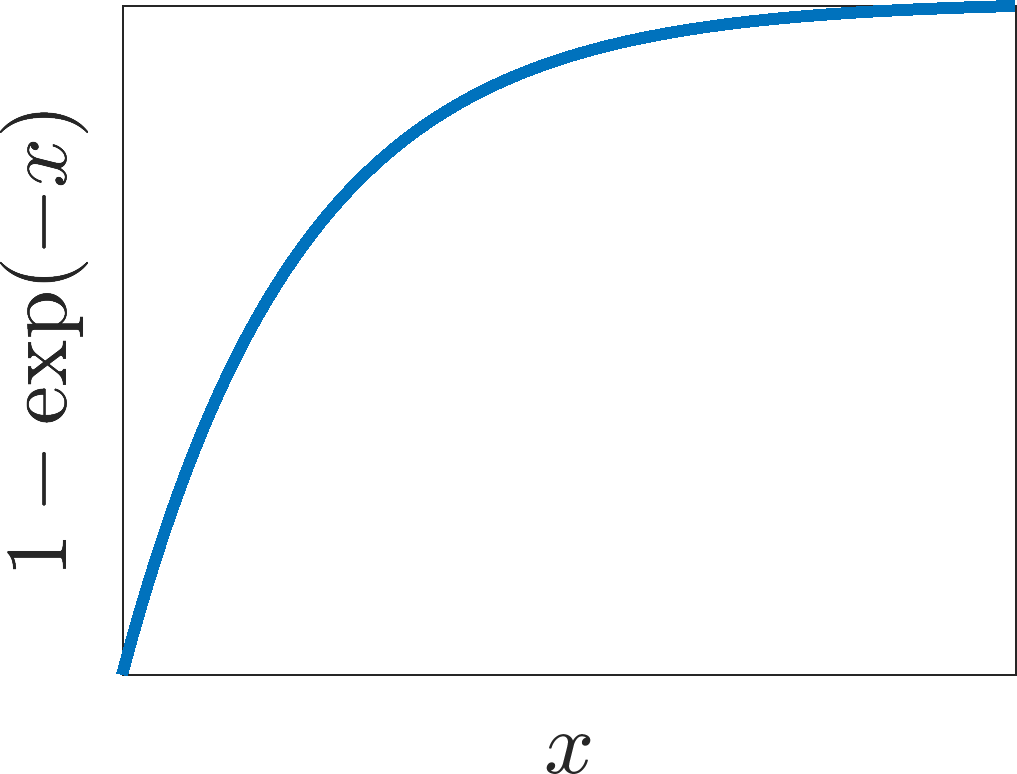
\includegraphics[width=\tttp]{../Pictures/Strictly_monotonic.png}}
\caption{\label{Monotonics}(a)\COL{ A non-monotonic function.} (b) \COL{A monotonic function.} (c) \COL{A strictly monotonic function.}}
\end{figure}


\begin{cor}
Suppose $F(u)$ is a scalar function that is continuously differentiable. The solution, $u(t)$, of the one dimensional ODE,
\bb
\dot{u}=F(u),\quad u(t_0)=u_0,
\ee
cannot oscillate. Specifically, $u(t)$ must either be constant, or a monotonically increasing, or decreasing function.
\end{cor}
\begin{proof}
\COL{Suppose that $u^*(t)$ is non-monotonic. By definition its derivative changes sign. By continuity there is somewhere, $t_c$, such that $\rd u^*(t_c)/\rd t=0$.
Thus, $u^*$ is a solution of
\bb
\dot{u^*}=F(u^*),\quad u^*(t_c)=u^*_c.\label{Starred}
\ee
Let us construct the constant function $u\equiv u^*_c$. We note that, $F(u^*(t_c))=0$ and, thus,  $u$ is also a solution to \eqn{Starred}. However, this means that we have two different solutions to \eqn{Starred} violating theorem \ref{Existence_Uniqueness}. By contradiction $u^*(t)$ has to be monotonic.}
\end{proof}
This means that to have oscillatory phenomena in a system either we need more than one population, or the system has to be non-autonomous. See example \ref{Duffing_example} for a case where both of these factors are present and do indeed produce oscillations (and chaos).



\section{Taylor expansions}
This section is to remind you of the Taylor expansion technique. The Taylor expansion is one of the most powerful tools for an applied mathematician because very often we want to know what happens to a trajectory near some critical point. Although the kinetics maybe very non-linear and difficult to understand globally we can use the Taylor expansion to simplify the dynamics in a small region around the critical point in order to gain knowledge about the dynamics in this region.

\begin{thm}\label{Taylor}
Suppose $f(x)$ is infinitely differentiable at a point $a$ then the Taylor series of $f$ at $a$ is the power series
\bb
f(x)=\sum _{n=0}^{\infty }{\frac{f^n(a)}{n!}(x-a)^n},
\ee
which is explicitly
\bb
f(x)=f(a)+{\frac {f'(a)}{1!}}(x-a)+{\frac {f''(a)}{2!}}(x-a)^{2}+{\frac {f'''(a)}{3!}}(x-a)^{3}+\cdots,
\ee
where $n!$ denotes the factorial of $n$ and $f^{(n)}(a)$ denotes the $n^{th}$ derivative of $f$ evaluated at the point $a$. The derivative of order zero of $f$ is defined to be $f$ itself and $(x-a)^0$ and $0!$ are both defined to be 1.
\end{thm}
\begin{example}[frametitle=Taylor expansions.]
\begin{itemize}
\item $\exp(x)$ at $x=0$ \see{Taylor_approximations}.
\COL{
\bb
\exp(x)=1+x+{\frac {1}{2}}{x}^{2}+{\frac {1}{6}}{x}^{3}+O \left( {x}^{4}
 \right) .
 \ee}
\item $\cos(x)$ at $x=0$.
\COL{
\bb
\cos(x)=1-{\frac {1}{2}}{x}^{2}+O \left( {x}^{4} \right) .
\ee}
\item $1/\l 1+x\r$ at $x=0$
\COL{
\bb
\frac{1}{1+x}=1-x+{x}^{2}-{x}^{3}+O \left( {x}^{4} \right) .
\ee}
\item $\sin(x)$ at $x=\pi/2$.
\COL{
\bb
\sin(x)=1-{\frac{1}{2}} \left( x-{\frac {\pi}{2}} \right) ^{2}+O \left( 
 \left( x-{\frac {\pi}{2}} \right) ^{4} \right)  .
\ee}
\end{itemize}
\end{example}
\begin{figure}[!!!h!!!tb]
\centering
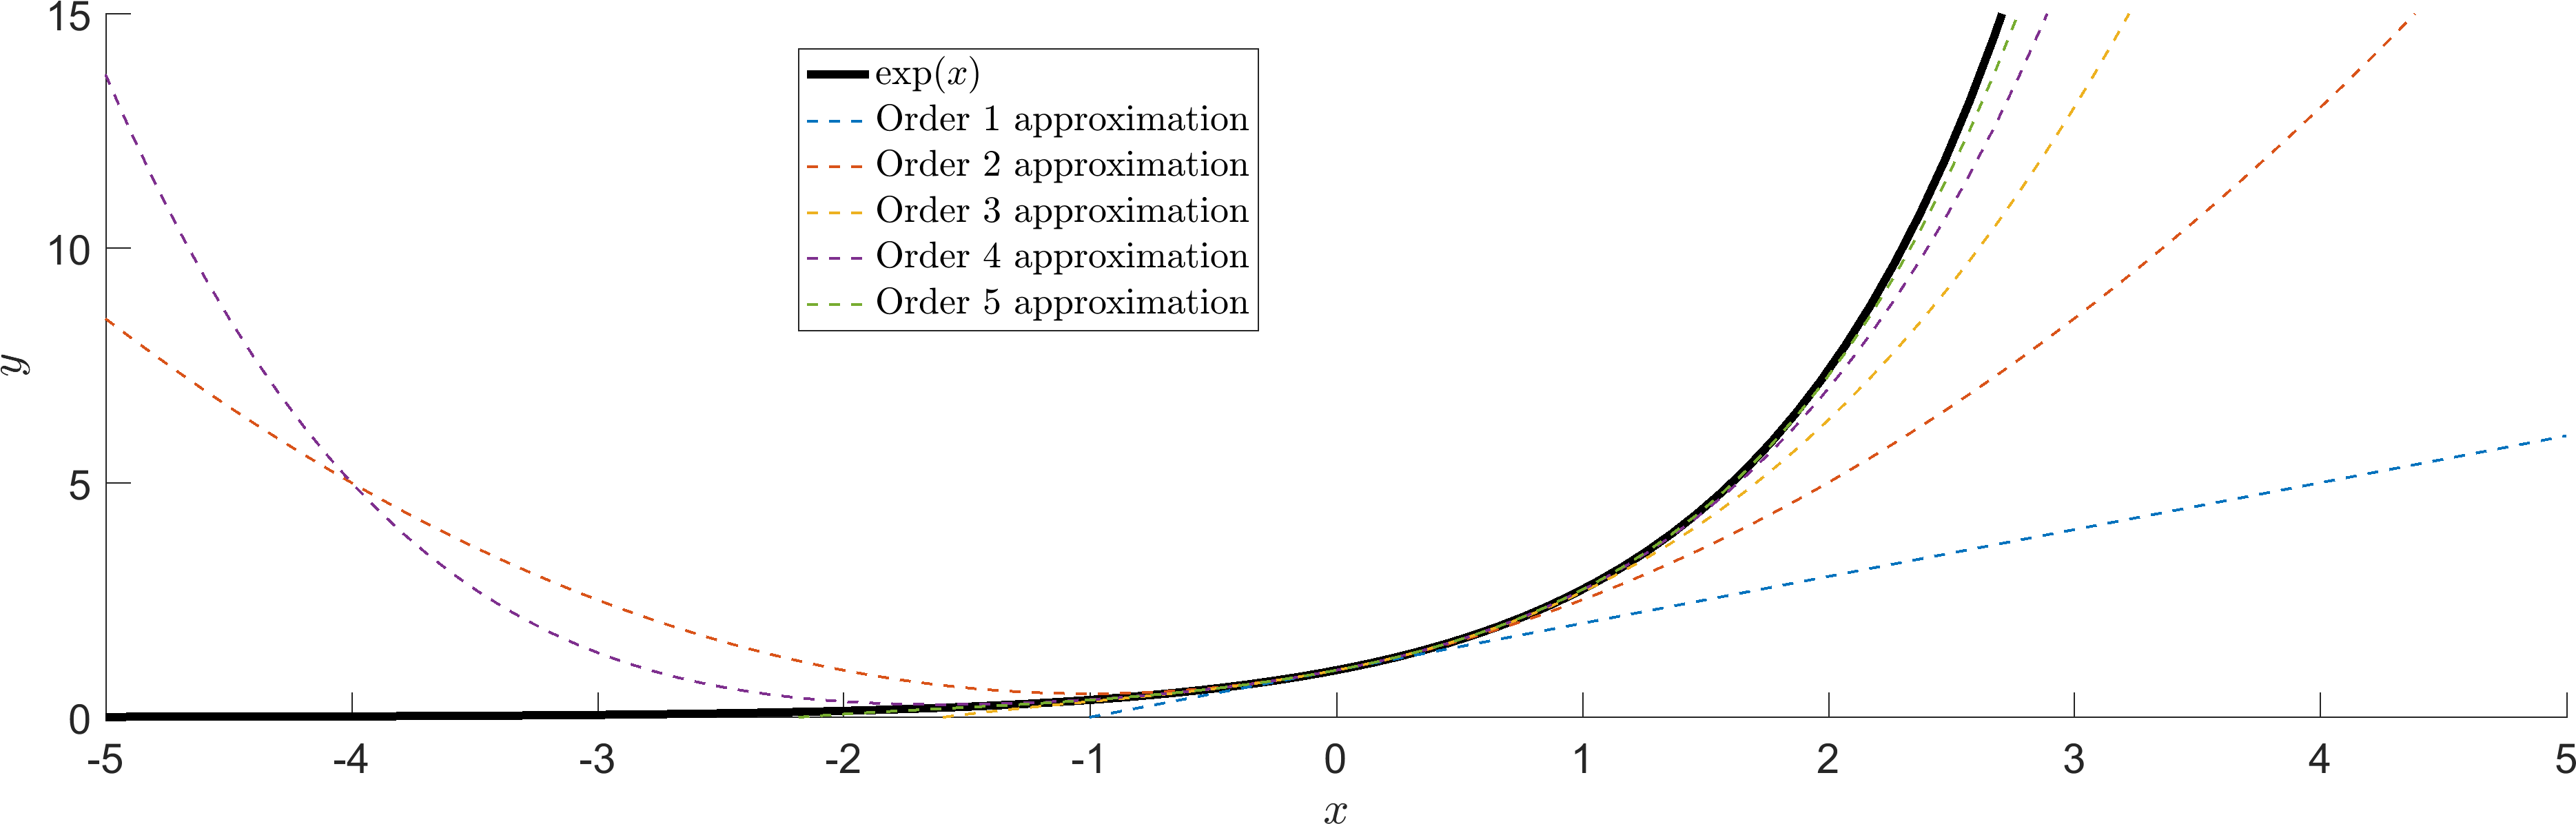
\includegraphics[width=\textwidth]{../Pictures/Taylor_approximations.png}
\caption{\label{Taylor_approximations} Approximating the exponential function with different orders of Taylor series.}
\end{figure}

\COL{Although Theorem \ref{Taylor} is the most general form of Taylor's theorem we are frequently going to want to know what happens near a specific point. Namely, if $x$ is the point of interest, what does the function look like at $x+\epsilon$, where $\epsilon \ll 1$. Specifically, this simply comes down to redefining $x\coloneqq x+\epsilon$ and $a\coloneqq x$ in Theorem \ref{Taylor}, namely
\bb
f(x+\epsilon)=f \left( x \right) +\epsilon{\frac {\rm d}{{\rm d}x}}f \left( x \right) 
+{\frac {{\epsilon}^{2}}{2}{\frac {{\rm d}^{2}}{{\rm d}{x}^{2}}}f \left( x
 \right) }+{\frac {{\epsilon}^{3}}{6}{\frac {{\rm d}^{3}}{{\rm d}{x}^{
3}}}f \left( x \right) }+O \left( {\epsilon}^{4}
 \right). 
\ee}\COL{
Since $\epsilon\ll 1$ we can truncate this series to obtain a good estimate after only a first term in $\epsilon$,
\bb
f(x+\epsilon)\approx f \left( x \right) +\epsilon{\frac {\rm d}{{\rm d}x}}f \left( x \right).
\ee
This is known as linearisation. You are taking the (possibly complicated) function $f$ and rewriting it as a linear function in $\epsilon$.}

Courses in the third year will deal with what information you get in the case that you truncate at $\epsilon^2$, or higher. This is non-linear analysis.

\subsection{Multivariate Taylor expansion}
A similar theorem can be stated when the function $f$ has more than one argument.
\begin{defin}
If $f$ is a function of more than one variable it is called \textbf{multivariate}.
\end{defin}

\COL{Here we simply state the expansion to first order expansion that we will be concerned with throughout the course.
\bb
f(x+\epsilon_1,y+\epsilon_2)\approx f(x,y)+\epsilon_1 f_x+\epsilon_2 f_y,
\ee
where we observe that we have used a subscript $f_x$ to denote the partial derivative $\partial f/\partial x$ and similarly for $f_y$.}
\begin{defin}
For brevity we use subscripts to stand for partial derivatives,
\bb
f_{x_1x_2\dots x_n}=\frac{\partial^n f}{\partial x_1\partial x_2\dots\partial x_n}.
\ee
\end{defin}
\begin{example}[frametitle=Multivariate Taylor expansion.]
\begin{itemize}
\item $\sin(x+y)$ at $x=y=0$.
\COL{
\bb
\sin(x+y)\approx x+y.
\ee}
\item $\sin(x)\cos(y)$ at $x=y=0$.
\COL{
\bb
\sin(x)\cos(y)\approx x.
\ee}
\end{itemize}
\end{example}

\section{Polar coordinates}
Many phenomena that we will model will fall under the consideration of spatial movement, for example in Chapter \ref{How to model a system} and question sheet two we will be considering planetary movement. Critically, in many of these cases the objects tend to move in circular trajectories orbiting a single point. Thus, it is more natural to use polar coordinates $(r,\theta)$ to describe the motion, rather than Cartesian coordinates $(x,y)$ \see{Polars}. However, it may be easier to model the system in Cartesian coordinates. Thus, we need to know how to convert between one set and another.
\begin{figure}[h!!!tb]
\centering
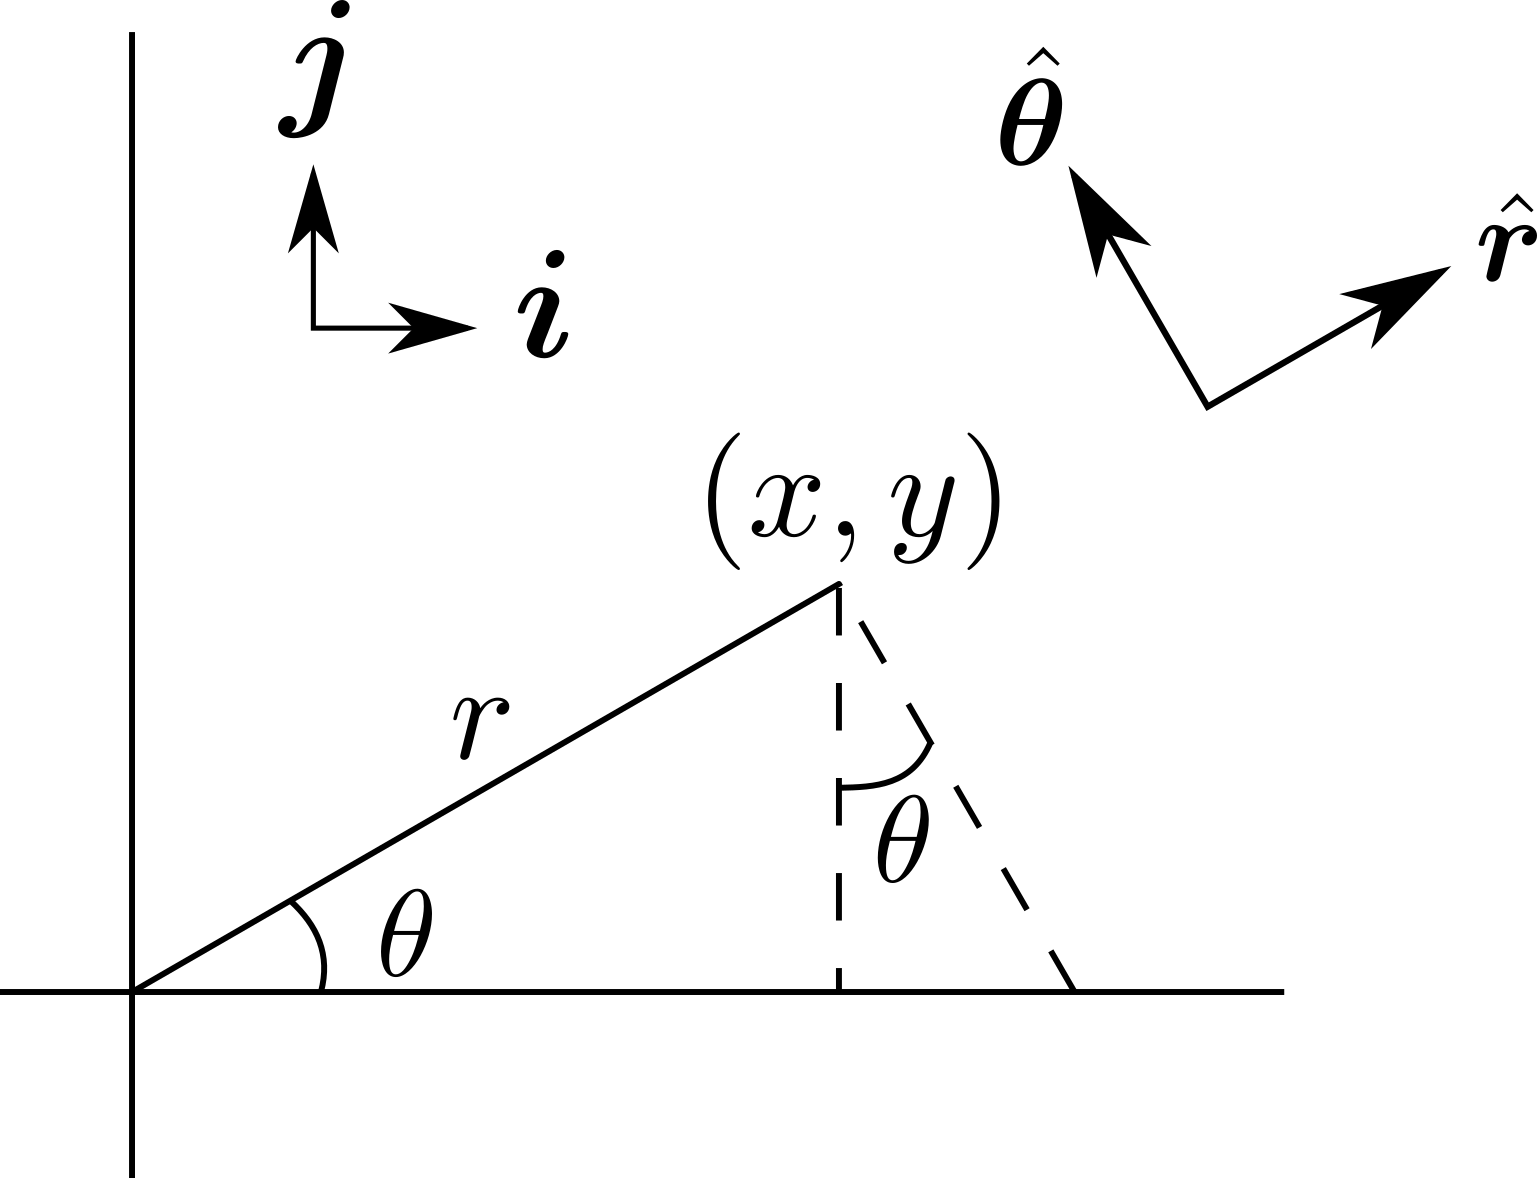
\includegraphics[width=\ttp]{../Pictures/Polars.png}
\caption{\label{Polars} Cartesian and polar coordinates.}
\end{figure} 

\fig{Polars} illustrates the fundamental relationships between the Cartesian and the polar coordinates, namely:
\begin{align}
x=r\cos(\theta),\\
y=r\sin(\theta).
\end{align}
Critically, these specify $x$ and $y$ singly as functions $(r,\theta)$. These, in turn, can be used to construct equations for $r$ and $\theta$ separately as functions of $(x,y)$, namely,
\bb
r^2=x^2+y^2,
\ee
and
\bb
\theta=\arctan\l\frac{y}{x}\r,\quad \textrm{or}\quad\theta=\arccos\l\frac{x}{\sqrt{x^2+y^2}}\r,\quad \textrm{or}\quad\theta=\arcsin\l\frac{y}{\sqrt{x^2+y^2}}\r.\label{theta_eqns}
\ee
where the appropriate function $\theta(x,y)$ is chosen depending on which ever is easiest to use.

\begin{example}[frametitle=Cartesian to polar conversion.]
\COL{Suppose
\begin{align}
\dot{x}&=f(x,y),\\
\dot{y}&=g(x,y)
\end{align}
how do we convert the system from Cartesian coordinates to polar coordinates?

First we use the condition that $r^2=x^2+y^2$. Taking derivatives we get
\bb
2r\dot{r}=2x\dot{x}+2y\dot{y}.
\ee
At which point we can exchange all Cartesian coordinates for their polar analogues, namely:
\bb
\dot{r}=\cos(\theta)f(r\cos(\theta),r\sin(\theta))+\sin(\theta)g(r\cos(\theta),r\sin(\theta)).
\ee
Next we need $\dot{\theta}$. Since there are multiple (equivalent) ways of representing $\theta$ there are multiple (equivalent) forms of the derivative, here only one will be presented. Other forms follow exactly the same procedure. We note that
\bb
\dot{x}=f(r\cos(\theta),r\sin(\theta))=\frac{\rd \l r\cos(\theta)\r}{\rd t}=\dot{r}\cos(\theta)-r\sin(\theta)\dot{\theta}.\label{xdot_to_r}
\ee
}\COL{Rearranging \eqn{xdot_to_r} gives
\begin{align}
\dot{\theta}&=\frac{\cos(\theta)^2f+\sin(\theta)\cos(\theta)g-f}{r\sin(\theta)},\\
&=\frac{-\sin(\theta)f+\sin(\theta)\cos(\theta)g}{r\sin(\theta)},\\
&=\frac{\cos(\theta)g-f\sin(\theta)}{r}.
\end{align}
where the arguments of $f$ and $g$ have been suppressed for brevity.}
\end{example}

In the above example we created $\dot{r}$ first and then used this to produce $\dot{\theta}$. In following example we show how to do the substitution all in one go.
\begin{example}[frametitle= A quicker conversion]
\COL{From
\begin{align}
x=r\cos(\theta),\\
y=r\sin(\theta).
\end{align}
we generate
\begin{align}
&\dot{x}=f(x,y)=\dot{r}\cos(\theta)-r\sin(\theta)\dot{\theta},\\
&\dot{y}=g(x,y)=\dot{r}\sin(\theta)+r\cos(\theta)\dot{\theta}.
\end{align}
This can be seen as a set of simultaneous equations and, thus, solved as a matrix problem
\bb
\colvec{2}{f}{g}=\begin{pmatrix}
\cos(\theta)& -r\sin(\theta) \\
\sin(\theta) & r\cos(\theta)
\end{pmatrix}
\colvec{2}{\dot{r}}{\dot{\theta}}.
\ee
The matrix can be inverted to produce
\bb
\frac{1}{r}\begin{pmatrix}
r\cos(\theta)& r\sin(\theta) \\
-\sin(\theta) & \cos(\theta)
\end{pmatrix}\colvec{2}{f}{g}=
\colvec{2}{\dot{r}}{\dot{\theta}},
\ee
which allows us to reproduce
\bb
\dot{r}=\cos(\theta)f+\sin(\theta)g.
\ee
\bb
\dot{\theta}=\frac{\cos(\theta)g-f\sin(\theta)}{r}.
\ee
}
\end{example}
Generally, nonlinear equations are not solvable however, we will see in the next example the polar coordinates can convert nonlinearities in $(x,r)$ to linearities in $(r,\theta)$
\begin{example}[frametitle= Solving ODEs in polar coordinates]
\COL{Consider the following system
\begin{align}
\dot{x}=y+x\l 1-x^2-y^2\r,\label{x_polar}\\
\dot{y}=-x+y\l 1-x^2-y^2\r\label{y_polar}.
\end{align}
Convert to polar coordinates
\begin{align}
\dot{r}&=\frac{xy+x^2\l 1-x^2-y^2\r-xy+y^2\l 1-x^2-y^2\r}{r},\\
&=\frac{(x^2+y^2)\l 1-x^2-y^2\r}{r},\\
&=r(1-r^2).
\end{align}
and
\bb
\dot{x}=y+x\l 1-x^2-y^2\r=\dot{r}\cos(\theta)-r\sin(\theta)\dot{\theta},
\ee
which implies
\begin{align}
\dot{\theta}&=\frac{\dot{r}\cos(\theta)-y-x\l 1-x^2-y^2\r}{r\sin(\theta)},\\
&=\frac{r(1-r^2)\cos(\theta)-r\sin(\theta)-r\cos(\theta)(1+r^2)}{r\sin(\theta)},\\
&=-1.
\end{align}
Assuming initial conditions $\theta(0)=0$ and $r(0)=r_0>0$ we can immediately integrate to get $\theta=-t$ and
\begin{align}
t&=\int^r_{r_0}\frac{1}{r'(1-r'^2)}\rd r',\\
&=\int^r_{r_0}\frac{1}{r'}+\frac{1/2}{1-r'}-\frac{1/2}{1+r'}\rd r',\\
&=\left[\frac{1}{r'}+\frac{1/2}{1-r'}-\frac{1/2}{1+r'}\right]^r_{r_0},\\
&=\left[\ln(r')-1/2\ln(1-r')-1/2\ln(1+r')\right]^r_{r_0},\\
&=\left[\ln\l \frac{r'}{\sqrt{1-r'^2}}\r\right]^r_{r_0},\\
&=\ln\l \frac{r}{\sqrt{1-r^2}}\frac{\sqrt{1-r_0^2}}{r_0}\r,
\end{align}

Rearranging this gives,
\bb
r(t)=\frac{r_0}{\sqrt{r_0^2+e^{-2t}\l 1-r_0^2\r}}.\label{r_lim}
\ee
From \eqn{r_lim} we can see that $r(t)\rightarrow 1$ as $t\rightarrow \infty$. Critically, we can reconstruct the Cartesian solution by considering the polar identities. Firstly, since $\theta=-t$ the solutions spiral at a constant rate. Note the spirals go clockwise as we normally take positive angles to be anticlockwise. Further, any trajectory must head towards the circle $r=1$.

The full dynamics are simulated in \fig{Polar_plot}
}
\end{example}
\begin{figure}[h!!!tb]
\centering
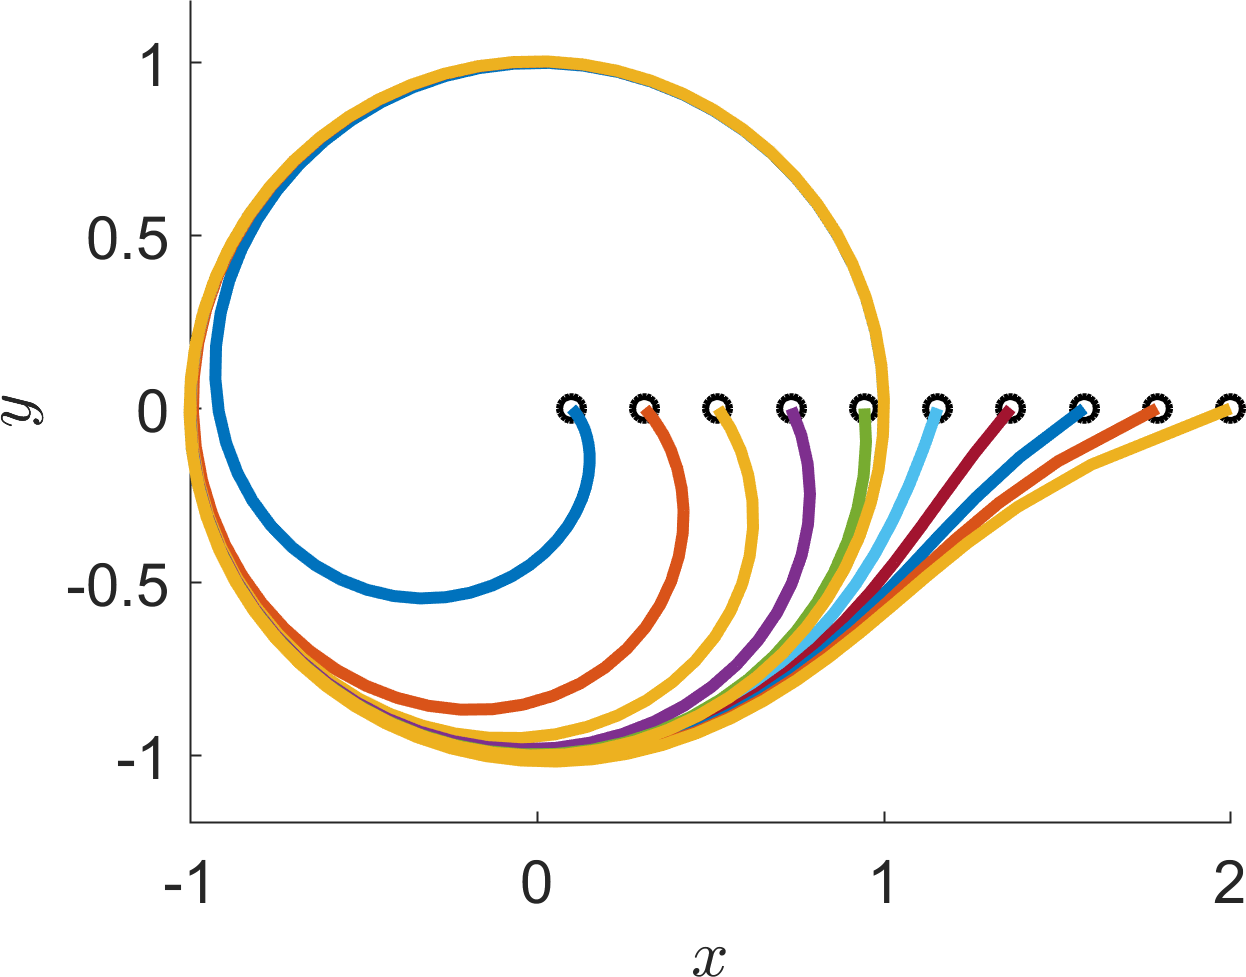
\includegraphics[width=\ttp]{../Pictures/Polar_plot.png}
\caption{\label{Polar_plot} Full dynamics of \eqns{x_polar}{y_polar}.}
\end{figure} 
\section{Check list}
By the end of this chapter you should be able to:
\begin{todolist}
\item reproduce all the definitions;
\item state all theorems;
\item solve simple linear ODE systems;
\item prove trajectories of autonomous systems cannot cross themselves;
\item prove that an ODE of one variable cannot oscillate;
\item derive single variable Taylor series of any order;
\item derive multivariate Taylor series up to first order;
\item convert systems of ODE equations of Cartesian variables in to polar variables and back again.
\end{todolist}




